%% LyX 2.3.6.2 created this file.  For more info, see http://www.lyx.org/.
%% Do not edit unless you really know what you are doing.
\documentclass[english]{beamer}
\usepackage[T1]{fontenc}
\usepackage[latin9]{inputenc}
\setcounter{secnumdepth}{3}
\setcounter{tocdepth}{3}
\usepackage{babel}
\usepackage{graphicx}
\ifx\hypersetup\undefined
  \AtBeginDocument{%
    \hypersetup{unicode=true,pdfusetitle,
 bookmarks=true,bookmarksnumbered=false,bookmarksopen=false,
 breaklinks=false,pdfborder={0 0 1},backref=false,colorlinks=true}
  }
\else
  \hypersetup{unicode=true,pdfusetitle,
 bookmarks=true,bookmarksnumbered=false,bookmarksopen=false,
 breaklinks=false,pdfborder={0 0 1},backref=false,colorlinks=true}
\fi

\makeatletter

%%%%%%%%%%%%%%%%%%%%%%%%%%%%%% LyX specific LaTeX commands.
%% Because html converters don't know tabularnewline
\providecommand{\tabularnewline}{\\}

%%%%%%%%%%%%%%%%%%%%%%%%%%%%%% Textclass specific LaTeX commands.
% this default might be overridden by plain title style
\newcommand\makebeamertitle{\frame{\maketitle}}%
% (ERT) argument for the TOC
\AtBeginDocument{%
  \let\origtableofcontents=\tableofcontents
  \def\tableofcontents{\@ifnextchar[{\origtableofcontents}{\gobbletableofcontents}}
  \def\gobbletableofcontents#1{\origtableofcontents}
}
\newenvironment{lyxcode}
  {\par\begin{list}{}{
    \setlength{\rightmargin}{\leftmargin}
    \setlength{\listparindent}{0pt}% needed for AMS classes
    \raggedright
    \setlength{\itemsep}{0pt}
    \setlength{\parsep}{0pt}
    \normalfont\ttfamily}%
   \def\{{\char`\{}
   \def\}{\char`\}}
   \def\textasciitilde{\char`\~}
   \item[]}
  {\end{list}}

%%%%%%%%%%%%%%%%%%%%%%%%%%%%%% User specified LaTeX commands.
\usetheme[secheader]{Boadilla}
\usecolortheme{seahorse}
\title[What I learned about FP]{What I learned about functional programming}
\subtitle{while writing a book on it}
\author{Sergei Winitzki}
\date{2021-10-29}
\institute[SBTB]{Scale by the Bay 2021}
\setbeamertemplate{headline}{} % disable headline at top
\setbeamertemplate{navigation symbols}{} % disable navigation bar at bottom
\usepackage[all]{xy} % xypic
%\makeatletter
% Macros to assist LyX with XYpic when using scaling.
\newcommand{\xyScaleX}[1]{%
\makeatletter
\xydef@\xymatrixcolsep@{#1}
\makeatother
} % end of \xyScaleX
\makeatletter
\newcommand{\xyScaleY}[1]{%
\makeatletter
\xydef@\xymatrixrowsep@{#1}
\makeatother
} % end of \xyScaleY

% Double-stroked fonts to replace the non-working \mathbb{1}.
\usepackage{bbold}
\DeclareMathAlphabet{\bbnumcustom}{U}{BOONDOX-ds}{m}{n} % Use BOONDOX-ds or bbold.
\newcommand{\custombb}[1]{\bbnumcustom{#1}}
% The LyX document will define a macro \bbnum{#1} that calls \custombb{#1}.

\usepackage{relsize} % make math symbols larger or smaller
\usepackage{stmaryrd} % some extra symbols such as \fatsemi
% Note: using \forwardcompose inside a \text{} will cause a LaTeX error!
\newcommand{\forwardcompose}{\hspace{1.5pt}\ensuremath\mathsmaller{\fatsemi}\hspace{1.5pt}}


% Make underline green.
\definecolor{greenunder}{rgb}{0.1,0.6,0.2}
%\newcommand{\munderline}[1]{{\color{greenunder}\underline{{\color{black}#1}}\color{black}}}
\def\mathunderline#1#2{\color{#1}\underline{{\color{black}#2}}\color{black}}
% The LyX document will define a macro \gunderline{#1} that will use \mathunderline with the color `greenunder`.
%\def\gunderline#1{\mathunderline{greenunder}{#1}} % This is now defined by LyX itself with GUI support.

% Scala syntax highlighting. See https://tex.stackexchange.com/questions/202479/unable-to-define-scala-language-with-listings
%\usepackage[T1]{fontenc}
%\usepackage[utf8]{inputenc}
%\usepackage{beramono}
%\usepackage{listings}
% The listing settings are now supported by LyX in a separate section "Listings".
\usepackage{xcolor}

\definecolor{scalakeyword}{rgb}{0.16,0.07,0.5}
\definecolor{dkgreen}{rgb}{0,0.6,0}
\definecolor{gray}{rgb}{0.5,0.5,0.5}
\definecolor{mauve}{rgb}{0.58,0,0.82}
\definecolor{aqua}{rgb}{0.9,0.96,0.999}
\definecolor{scalatype}{rgb}{0.2,0.3,0.2}
\usepackage[nocenter]{qtree}
\usepackage{relsize}
\renewcommand\arraystretch{1.4}

\makeatother

\usepackage{listings}
\lstset{language=Scala,
morekeywords={{scala}},
otherkeywords={=,=>,<-,<\%,<:,>:,\#,@,:,[,],.,???},
keywordstyle={\color{scalakeyword}},
morekeywords={[2]{String,Short,Int,Long,Char,Boolean,Double,Float,BigDecimal,Seq,Map,Set,List,Option,Either,Future,Vector,Range,IndexedSeq,Try,true,false,None,Some,Left,Right,Nothing,Any,Array,Unit,Iterator,Stream}},
keywordstyle={[2]{\color{scalatype}}},
frame=tb,
aboveskip={1.5mm},
belowskip={0.5mm},
showstringspaces=false,
columns=fullflexible,
keepspaces=true,
basicstyle={\smaller\ttfamily},
extendedchars=true,
numbers=none,
numberstyle={\tiny\color{gray}},
commentstyle={\color{dkgreen}},
stringstyle={\color{mauve}},
frame=single,
framerule={0.0mm},
breaklines=true,
breakatwhitespace=true,
tabsize=3,
framexleftmargin={0.5mm},
framexrightmargin={0.5mm},
xleftmargin={1.5mm},
xrightmargin={1.5mm},
framextopmargin={0.5mm},
framexbottommargin={0.5mm},
fillcolor={\color{aqua}},
rulecolor={\color{aqua}},
rulesepcolor={\color{aqua}},
backgroundcolor={\color{aqua}},
mathescape=false,
extendedchars=true}
\renewcommand{\lstlistingname}{Listing}

\begin{document}
\global\long\def\gunderline#1{\mathunderline{greenunder}{#1}}%
\global\long\def\bef{\forwardcompose}%
\global\long\def\bbnum#1{\custombb{#1}}%
\frame{\titlepage}
\begin{frame}{Why write a book about functional programming. I}

My background: theoretical physics
\begin{itemize}
\item I used to write academic papers with lots of formulas and diagrams\vspace{-0.3\baselineskip}
\end{itemize}
\begin{center}
\includegraphics[width=0.25\columnwidth]{\string"Winitzki - conformal diagrams - sample page\string".png}\includegraphics[height=0.47\textheight]{\string"Winitzki - physics paper - sample page\string".png}\includegraphics[width=0.2\columnwidth]{\string"Winitzki - eibook - sample page\string".png}\vspace{-0.6\baselineskip}
\par\end{center}
\begin{itemize}
\item Repented and turned to software engineering in 2010
\end{itemize}
I have been studying FP since 2008 (OCaml, Haskell, Scala)
\begin{itemize}
\item Learning from papers, online tutorials, and books
\item Attending the SBTB conferences since 2014
\item Using Scala at my day job since 2015
\end{itemize}
\end{frame}

\begin{frame}{Why write a book about functional programming. II}

I found the FP community to be unlike other programmers' communities
\begin{itemize}
\item Others are focused on a chosen programming language (Java, Python,
JavaScript, etc.), and on designing and using libraries and frameworks
\begin{itemize}
\item \emph{``use this framework, override this method, use this annotation''}
\end{itemize}
\item The FP community talks in a very different way
\begin{itemize}
\item \emph{``referential transparency, algebraic data types, monoid laws,
parametric polymorphism, free applicative functors, monad transformers,
Yoneda lemma, Curry-Howard isomorphism, profunctor lenses, catamorphisms''}
\begin{itemize}
\item \href{https://degoes.net/articles/fp-glossary}{A glossary of FP terminology}
(more than $100$ terms)
\end{itemize}
\item From SBTB 2018: \emph{\href{https://www.youtube.com/watch?v=L0aYcq1tqMo}{The Functor,  Applicative,  Monad talk}}
\begin{itemize}
\item By 2018, everyone expects to hear a talk about these concepts
\end{itemize}
\item An \href{https://stackoverflow.com/questions/36002541/mysterious-gadt-skolem-what-type-is-trying-to-escape-its-scope}{actual Scala error message}:
\end{itemize}
\end{itemize}
\begin{lyxcode}
\textcolor{blue}{\footnotesize{}found~~~:~Seq{[}Some{[}V{]}{]}}{\footnotesize\par}

\textcolor{blue}{\footnotesize{}required:~Seq{[}Option{[}?V8{]}{]}~where~type~?V8~<:~V~(this~is~a~GADT~skolem)}{\footnotesize\par}
\end{lyxcode}
To do FP, should I learn all of this? How do I learn about this?
\end{frame}

\begin{frame}{Why write a book about functional programming. III}

Main questions:
\begin{itemize}
\item Which theoretical knowledge will actually help write Scala code?
\item Where can one learn this FP theory, with definitions and examples?
\end{itemize}
What I did \emph{not} want to see:
\begin{itemize}
\item Heuristic explanations without derivations and proofs
\begin{itemize}
\item Most FP books show code without proofs or rigorous definitions
\begin{itemize}
\item \emph{\href{https://www.amazon.com/Book-Monads-Alejandro-Serrano-Mena/dp/0578405296}{The Book of Monads}}
does not prove the laws for any monads
\end{itemize}
\item A few books (\href{https://en.wikibooks.org/wiki/Haskell}{Haskell Wikibooks}\emph{,
\href{https://www.amazon.co.uk/Introduction-Functional-Programming-Prentice-Hall-Paperback/dp/B00OVNLJTS/}{Introduction to functional programming using Haskell},}
and \emph{\href{https://www.manning.com/books/functional-programming-in-scala}{Functional programming in Scala}})
include some simple proofs
\end{itemize}
\item Academic theory for the sake of theory, with no applications
\begin{itemize}
\item ``\emph{\href{https://stackoverflow.com/questions/3870088/a-monad-is-just-a-monoid-in-the-category-of-endofunctors-whats-the-problem}{Monad is just a monoid in the category of endofunctors}}''
\item \emph{\href{https://www.amazon.com/Book-Monads-Alejandro-Serrano-Mena/dp/0578405296}{The Book of Monads}}
chapter 18 (adjunctions)
\item \href{https://bartoszmilewski.com/2017/08/26/lawvere-theories/}{Lawvere theories}
as an alternative to monads
\end{itemize}
\end{itemize}
\end{frame}

\begin{frame}{Why write a book about functional programming. IV}

Reading various materials has given me more questions than answers 

I started writing a \href{https://leanpub.com/sofp}{new book} to
answer all my FP questions
\begin{itemize}
\item by motivating and deriving all results from scratch
\item organizing systematically the practice-relevant parts of FP theory
\end{itemize}
{\small{}}%
\begin{minipage}[t]{0.78\columnwidth}%
\vspace{-0.4\baselineskip}
The book explains (with code examples and exercises):
\begin{itemize}
\item theory and applications of major design patterns of FP
\item techniques for deriving and verifying properties of types and code
(typeclass laws, equivalence of types)
\item practical motivations for (and applications of) these techniques
\end{itemize}
%
\end{minipage}{\small{}~ }%
\begin{minipage}[t][1\totalheight][c]{0.27\columnwidth}%
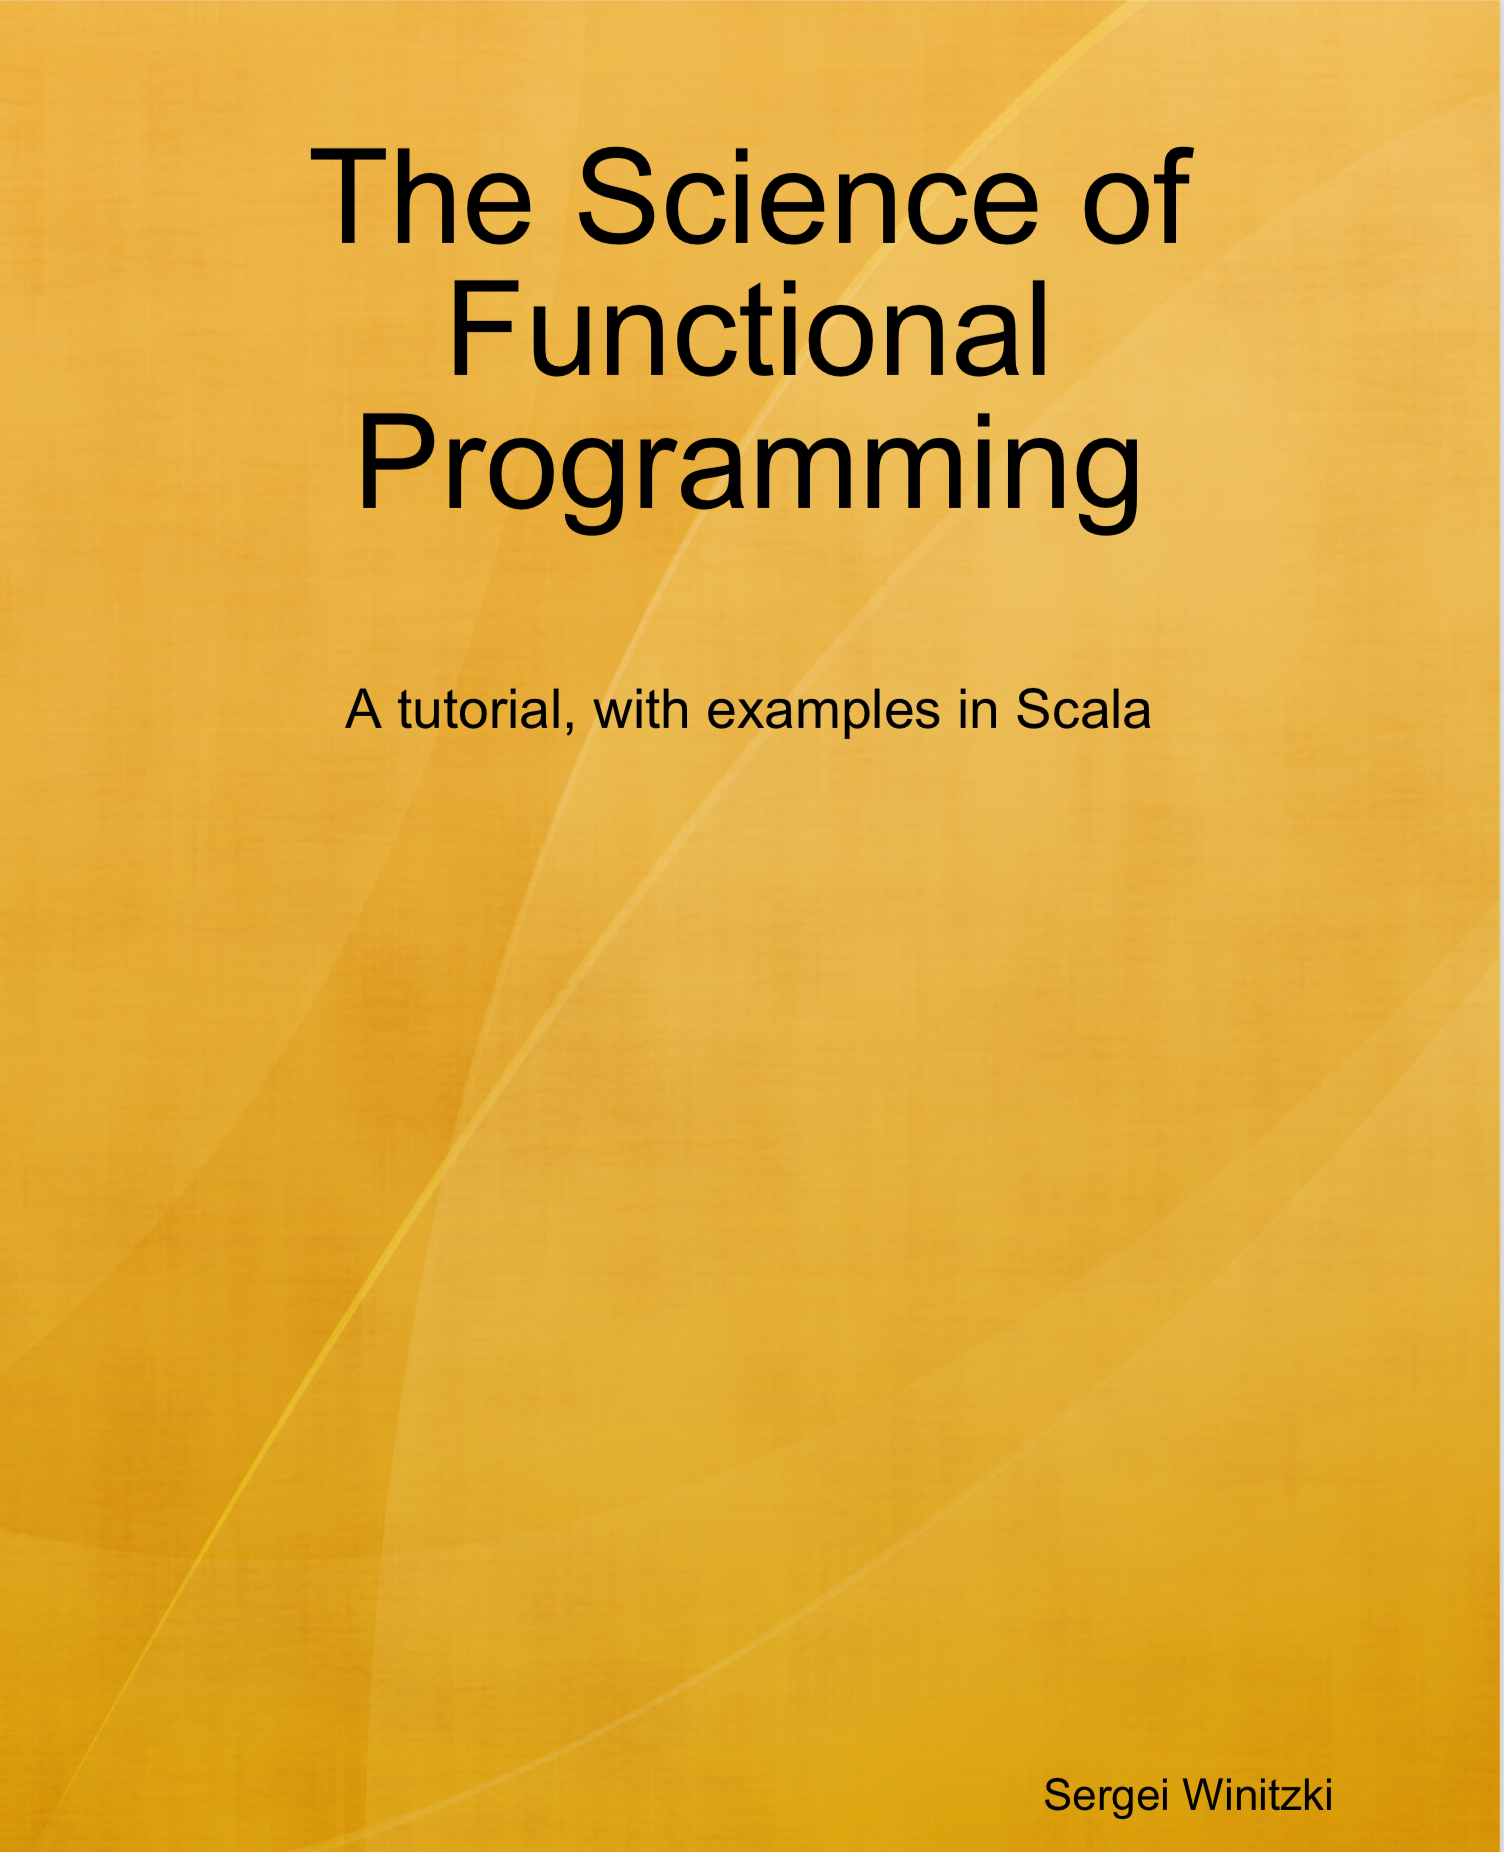
\includegraphics[width=2.5cm]{book-draft-cover}%
\end{minipage}{\small\par}

{\small{}Status of the book: 12.5 out of 14 chapters are ready}{\small\par}
\end{frame}

\begin{frame}{What I learned. I. Questions that have rigorous answers}

In FP, a programmer encounters certain questions about code that can
be answered rigorously 
\begin{itemize}
\item The answers will guide the programmer in designing the code
\item The answers are \emph{not} a matter of opinion or experience
\item The answers are found via mathematical derivations and reasoning
\end{itemize}
\end{frame}

\begin{frame}{Examples of reasoning tasks. I}

\begin{enumerate}
\item []\setcounter{enumi}{0}{\footnotesize{}\vspace{-0.4cm}}{\footnotesize\par}
\item Can we compute a value of type \texttt{\textcolor{blue}{\footnotesize{}Either{[}Z,
R => A{]}}} given a value of type \texttt{\textcolor{blue}{\footnotesize{}R
=> Either{[}Z, A{]}}} and conversely? (\texttt{\textcolor{blue}{\footnotesize{}A}},
\texttt{\textcolor{blue}{\footnotesize{}R}}, \texttt{\textcolor{blue}{\footnotesize{}Z}}
are type parameters.)
\end{enumerate}
\begin{lyxcode}
\textcolor{blue}{\footnotesize{}def~f{[}Z,~R,~A{]}(r:~R~=>~Either{[}Z,~A{]}):~Either{[}Z,~R~=>~A{]}~=~???}{\footnotesize\par}

\textcolor{blue}{\footnotesize{}def~g{[}Z,~R,~A{]}(e:~Either{[}Z,~R~=>~A{]}):~R~=>~Either{[}Z,~A{]}~=~???}{\footnotesize\par}
\end{lyxcode}
\begin{itemize}
\item We can implement \texttt{\textcolor{blue}{\footnotesize{}g}}, and
there is only one way:
\end{itemize}
\begin{lyxcode}
\textcolor{blue}{\footnotesize{}def~g{[}Z,~R,~A{]}(e:~Either{[}Z,~R~=>~A{]}):~R~=>~Either{[}Z,~A{]}~=}{\footnotesize\par}

\textcolor{blue}{\footnotesize{}~~r~=>~e.map(f~=>~f(r))~~~~~~~//~}{\footnotesize{}Scala~2.12~code}{\footnotesize\par}
\end{lyxcode}
\begin{itemize}
\item It turns out that \texttt{\textcolor{blue}{\footnotesize{}f}} \emph{cannot}
be implemented
\begin{itemize}
\item Not because we are insufficiently clever, but because... math!
\end{itemize}
\item Programmers need to develop intuition about why this is so
\item These results are rigorous
\begin{itemize}
\item The Curry-Howard isomorphism and the LJT algorithm
\item The code for \texttt{\textcolor{blue}{\footnotesize{}g{[}Z, R, A{]}}}
can be generated automatically
\end{itemize}
\end{itemize}
\end{frame}

\begin{frame}{Examples of reasoning tasks. II}

\begin{enumerate}
\item []\setcounter{enumi}{1}{\footnotesize{}\vspace{-0.4cm}}{\footnotesize\par}
\item How to use \texttt{\textcolor{blue}{\footnotesize{}for}} / \texttt{\textcolor{blue}{\footnotesize{}yield}}
with \texttt{\textcolor{blue}{\footnotesize{}Either{[}Z, A{]}}} and
\texttt{\textcolor{blue}{\footnotesize{}Future{[}A{]}}} together?
\end{enumerate}
\begin{lyxcode}
{\footnotesize{}\vspace{-0.15cm}}\textcolor{blue}{\footnotesize{}val~result~=~for~\{~//~This~code~will~not~compile;~need~to~combine...}{\footnotesize\par}

\textcolor{blue}{\footnotesize{}~~a~<-~Future(...)~//~~...~a~computation~that~is~run~asynchronously,}{\footnotesize\par}

\textcolor{blue}{\footnotesize{}~~b~<-~Either(...)~//~a~computation~whose~result~may~be~unavailable,}{\footnotesize\par}

\textcolor{blue}{\footnotesize{}~~c~<-~Future(...)~//~and~another~asynchronous~computation.}{\footnotesize\par}

\textcolor{blue}{\footnotesize{}\}~yield~???~~~~~//~Continue~computations~when~results~are~available.}{\footnotesize\par}
\end{lyxcode}
~~~~~\hspace*{1.8mm}Should \texttt{\textcolor{blue}{\footnotesize{}result}}
have type \texttt{\textcolor{blue}{\footnotesize{}Either{[}Z, Future{[}A{]}{]}}}
or \texttt{\textcolor{blue}{\footnotesize{}Future{[}Either{[}Z,A{]}{]}}}?

~~~~~\hspace*{1.8mm}How to combine \texttt{\textcolor{blue}{\footnotesize{}Either}}
with \texttt{\textcolor{blue}{\footnotesize{}Future }}so that we can
use \texttt{\textcolor{blue}{\footnotesize{}flatMap}}?
\begin{itemize}
\item It turns out that \texttt{\textcolor{blue}{\footnotesize{}Either{[}Z,
Future{[}A{]}{]}}} is wrong (cannot implement \texttt{\textcolor{blue}{\footnotesize{}flatMap}}
correctly). The correct type is \texttt{\textcolor{blue}{\footnotesize{}Future{[}Either{[}Z,
A{]}{]}}}.
\item Programmers need to develop intuition about why this is so
\item This is a rigorous result (programmers do not need to test it)
\begin{itemize}
\item The theory of monad transformers and their laws
\end{itemize}
\end{itemize}
\end{frame}

\begin{frame}{Examples of reasoning tasks. III}

\begin{enumerate}
\item []\setcounter{enumi}{2}{\footnotesize{}\vspace{-0.4cm}}{\footnotesize\par}
\item Can we implement \texttt{\textcolor{blue}{\footnotesize{}flatMap}}
for the type constructor \texttt{\textcolor{blue}{\footnotesize{}Option{[}(A,
A, A){]}}}?
\end{enumerate}
\begin{lyxcode}
\textcolor{blue}{\footnotesize{}def~flatMap{[}A,~B{]}(fa:~Option{[}(A,~A,~A){]})(f:~A~=>~Option{[}(B,~B,~B){]})}{\footnotesize\par}

\textcolor{blue}{\footnotesize{}~~~:~Option{[}(B,~B,~B){]}~=~???}{\footnotesize\par}
\end{lyxcode}
\begin{itemize}
\item It turns out that \texttt{\textcolor{blue}{\footnotesize{}flatMap}}
\emph{can} be implemented but fails the monad laws
\item Programmers need to develop intuition about why this is so
\begin{itemize}
\item How should we modify \texttt{\textcolor{blue}{\footnotesize{}Option{[}(A,
A, A){]}}} to make it into a monad?
\end{itemize}
\item This is a rigorous result (programmers do not need to test it)
\begin{itemize}
\item The theory of monads and their laws
\item The theory of type constructions of monads
\end{itemize}
\end{itemize}
\end{frame}

\begin{frame}{Examples of reasoning tasks. IV}

\begin{enumerate}
\item []\setcounter{enumi}{3}{\footnotesize{}\vspace{-0.4cm}}{\footnotesize\par}
\item Different people define a ``free monad'' via different sets of case
classes. Are these definitions equivalent? What is the difference?
\begin{itemize}
\item Three different implementations of the free monad: a \href{http://www.haskellforall.com/2012/06/you-could-have-invented-free-monads.html}{blog post}
by G.~Gonzalez (2012), a \href{http://functionaltalks.org/2014/11/23/runar-oli-bjarnason-free-monad/}{talk}
given by R.~Bjarnason (2014), and a \href{https://www.slideshare.net/KelleyRobinson1/why-the-free-monad-isnt-free-61836547}{talk}
given by K.~Robinson (2016) --- but no rigorous definitions
\end{itemize}
\end{enumerate}
\begin{itemize}
\item The free monad on a functor is less code than the free monad on a
non-functor
\item The free monad's encoding that assumes the monad laws is less code
than an encoding without assumed laws
\item These are rigorous results (programmers do not need to test them)
\begin{itemize}
\item The theory of ``free'' inductive typeclasses and their encodings
\end{itemize}
\item Programmers need intuition about implementing free typeclasses
\begin{itemize}
\item Given a \texttt{\textcolor{blue}{\footnotesize{}Pointed}} functor
(a functor that already has the \texttt{\textcolor{blue}{\footnotesize{}pure}}
method), implement a free monad or a free applicative 
\end{itemize}
\end{itemize}
\end{frame}

\begin{frame}{What I learned. II. Functional programming is engineering}

\begin{itemize}
\item FP is similar to engineering in some ways
\begin{itemize}
\item Mechanical, electrical, chemical engineering are based on calculus,
classical and quantum mechanics, electrodynamics, thermodynamics
\begin{itemize}
\item These sciences give engineers rigorous answers to certain questions
relevant to engineering design
\end{itemize}
\item FP is based on category theory, type theory, logic proof theory
\begin{itemize}
\item These theories give programmers rigorous answers to certain questions
relevant to writing code
\end{itemize}
\item Programming in non-FP paradigms is similar to \emph{artisanship} 
\end{itemize}
\item Engineers use special terminology
\begin{itemize}
\item Examples from mechanical, electrical, chemical engineering: \href{https://serc.carleton.edu/NAGTWorkshops/mineralogy/mineral_physics/tensors.html}{rank-4 tensors},
\href{https://arxiv.org/abs/math/0008147}{Lagrangians with non-holonomic constraints},
\href{https://www.youtube.com/watch?v=KAbqISZ6SHQ}{Fourier transform of the delta function},
\href{https://ocw.mit.edu/resources/res-6-008-digital-signal-processing-spring-2011/video-lectures/lecture-6-the-inverse-z-transform/}{inverse Z-transform},
\href{https://www.amazon.com/Introduction-Chemical-Engineering-Kinetics-Reactor/dp/1118368258}{Gibbs free energy}
\item Examples from FP: \href{https://wiki.haskell.org/Rank-N_types}{rank-$N$ types},
\href{https://www.cs.toronto.edu/~lczhang/324/ex/a2.pdf}{continuation-passing transformation},
\href{https://stackoverflow.com/questions/20152939/what-is-a-polymorphic-lambda}{polymorphic lambda functions},
\href{https://stackoverflow.com/questions/13352205/what-are-free-monads}{free monads},
\href{https://en.wikipedia.org/wiki/Hylomorphism_(computer_science)}{hylomorphisms}
\end{itemize}
\item As in engineering, the special terminology in FP is \emph{not} self-explanatory
\begin{itemize}
\item What is a delta function? What is a lambda function? 
\item What is the Gibbs free energy? What is the free monad?
\end{itemize}
\end{itemize}
\end{frame}

\begin{frame}{What I learned. III. The science of \texttt{map} / \texttt{filter}
/ \texttt{reduce}}

The \texttt{\textcolor{blue}{\footnotesize{}map}} / \texttt{\textcolor{blue}{\footnotesize{}filter}}
/ \texttt{\textcolor{blue}{\footnotesize{}reduce}} (MFR) programming
style --- iteration without loops
\begin{itemize}
\item Compute the list of all integers $n$ between 1 and 100 that can be
expressed as $n=p*q$ (with $2\leq p\leq q$) in exactly $4$ different
ways 
\end{itemize}
\begin{lyxcode}
\textcolor{blue}{\footnotesize{}scala>~(1~to~100).filter~\{~n~=>}{\footnotesize\par}

\textcolor{blue}{\footnotesize{}~~~~~|~~~(2~to~n).count(x~=>~n~\%~x~==~0~\&\&~x~{*}~x~<=~n)~==~4}{\footnotesize\par}

\textcolor{blue}{\footnotesize{}~~~~~|~\}}{\footnotesize\par}

\textcolor{blue}{\footnotesize{}res0:~IndexedSeq{[}Int{]}~=~Vector(36,~48,~80,~100)}{\footnotesize\par}
\end{lyxcode}
The MFR programming style is an FP success story
\begin{itemize}
\item Nameless functions (``lambdas'', ``closures'') are widely used
\begin{itemize}
\item and have been added to most programming languages by now
\end{itemize}
\item Essential methods: \texttt{\textcolor{blue}{\footnotesize{}map}},
\texttt{\textcolor{blue}{\footnotesize{}filter}}, \texttt{\textcolor{blue}{\footnotesize{}flatMap}},
\texttt{\textcolor{blue}{\footnotesize{}zip}}, \texttt{\textcolor{blue}{\footnotesize{}fold}}{\footnotesize\par}
\item Similar techniques work with parallel and stream processing (\lstinline!Spark!)
\item Similar techniques work with relational databases (\lstinline!Slick!) 
\end{itemize}
\end{frame}

\begin{frame}{What I learned. III. The science of \texttt{map} / \texttt{filter}
/ \texttt{reduce}}

Essential MFR methods: \texttt{\textcolor{blue}{\footnotesize{}map}},
\texttt{\textcolor{blue}{\footnotesize{}filter}}, \texttt{\textcolor{blue}{\footnotesize{}flatMap}},
\texttt{\textcolor{blue}{\footnotesize{}zip}}, \texttt{\textcolor{blue}{\footnotesize{}fold}}{\footnotesize\par}
\begin{itemize}
\item What data types other than \texttt{\textcolor{blue}{\footnotesize{}Seq{[}A{]}}}
can support these methods?
\begin{itemize}
\item Algebraic data types?
\item Trees and other recursive types? 
\item Perfect-shaped trees? {\scriptsize{}\Tree[ [ [ [ $a_1$ ] [ $a_2$ ] ] [ [ $a_3$ ] [ $a_4$ ] ] ] [ [ [ $a_5$ ] [ $a_6$ ] ] [ [ $a_7$ ] [ $a_8$ ] ] ] ] }
\item Which methods can be defined for \texttt{\textcolor{blue}{\footnotesize{}MyData{[}A{]}}}?
\end{itemize}
\begin{lyxcode}
\textcolor{blue}{\footnotesize{}type~MyData{[}A{]}~=~String~=>~Option{[}(String,~A){]}}{\footnotesize\par}
\end{lyxcode}
\end{itemize}
\end{frame}

\begin{frame}{What I learned. III. The science of \texttt{map} / \texttt{filter}
/ \texttt{reduce}}

A systematic approach to understanding FP via a study of MFR
\begin{itemize}
\item Determine the required laws of \texttt{\textcolor{blue}{\footnotesize{}map}},
\texttt{\textcolor{blue}{\footnotesize{}filter}}, \texttt{\textcolor{blue}{\footnotesize{}flatMap}},
\texttt{\textcolor{blue}{\footnotesize{}zip}}, \texttt{\textcolor{blue}{\footnotesize{}fold}}{\footnotesize\par}
\begin{itemize}
\item The laws express the programmers' expectations about code behavior
\item Define the corresponding typeclasses
\begin{itemize}
\item \texttt{\textcolor{blue}{\footnotesize{}map}} --- \texttt{\textcolor{blue}{\footnotesize{}Functor}},
\texttt{\textcolor{blue}{\footnotesize{}filter}} --- \texttt{\textcolor{blue}{\footnotesize{}Filterable}},
\texttt{\textcolor{blue}{\footnotesize{}flatMap}} --- \texttt{\textcolor{blue}{\footnotesize{}Monad}},
\texttt{\textcolor{blue}{\footnotesize{}zip}} --- \texttt{\textcolor{blue}{\footnotesize{}Applicative}},
\texttt{\textcolor{blue}{\footnotesize{}fold}} --- \texttt{\textcolor{blue}{\footnotesize{}Traversable}}{\footnotesize\par}
\end{itemize}
\end{itemize}
\item Find type constructions that preserve the typeclass laws
\begin{itemize}
\item If \texttt{\textcolor{blue}{\footnotesize{}P{[}A{]}}} and \texttt{\textcolor{blue}{\footnotesize{}Q{[}A{]}}}
are filterable functors then so is \texttt{\textcolor{blue}{\footnotesize{}Either{[}P{[}A{]},
Q{[}A{]}{]}}}{\footnotesize\par}
\item If \texttt{\textcolor{blue}{\footnotesize{}P{[}A{]}}} is a monad then
so is \texttt{\textcolor{blue}{\footnotesize{}Either{[}A, P{[}A{]}{]}}}{\footnotesize\par}
\item If \texttt{\textcolor{blue}{\footnotesize{}P{[}A{]}}} and \texttt{\textcolor{blue}{\footnotesize{}Q{[}A{]}}}
are monads then so is \texttt{\textcolor{blue}{\footnotesize{}(P{[}A{]},
Q{[}A{]})}}{\footnotesize\par}
\item If \texttt{\textcolor{blue}{\footnotesize{}P{[}A{]}}} is a contravariant
functor then \texttt{\textcolor{blue}{\footnotesize{}P{[}A{]} => A}}
is a monad
\item If \texttt{\textcolor{blue}{\footnotesize{}P{[}A{]}}} and \texttt{\textcolor{blue}{\footnotesize{}Q{[}A{]}}}
are applicative then so is \texttt{\textcolor{blue}{\footnotesize{}Either{[}P{[}A{]},
(A, Q{[}A{]}){]}}}{\footnotesize\par}
\begin{itemize}
\item I found many more type constructions of this kind
\end{itemize}
\item Sometimes it becomes necessary to define additional typeclasses
\begin{itemize}
\item Contravariant functor, contravariant filterable, contravariant applicative
\end{itemize}
\end{itemize}
\item Develop intuition about implementing lawful typeclass methods 
\item Develop intuition about data types that can have those methods
\begin{itemize}
\item ... and about data types that \emph{cannot} (and reasons why)
\end{itemize}
\item Develop notation and proof techniques for proving the laws
\end{itemize}
\end{frame}

\begin{frame}{What I learned. IV. The logic of types}

FP is not just ``programming with functions'': types play a central
role
\begin{itemize}
\item The compiler needs to check all types at compile time
\item The language needs to support certain type constructions
\end{itemize}
Most of FP use cases are based on only six type constructions:
\begin{itemize}
\item Unit type --- \texttt{\textcolor{blue}{\footnotesize{}Unit}}{\footnotesize\par}
\item Type parameters --- \texttt{\textcolor{blue}{\footnotesize{}f{[}A{]}(x)}}{\footnotesize\par}
\item Product types --- \texttt{\textcolor{blue}{\footnotesize{}(A, B)}}{\footnotesize\par}
\item Co-product types (``disjunctive union'' types) --- \texttt{\textcolor{blue}{\footnotesize{}Either{[}A,
B{]}}}{\footnotesize\par}
\item Function types --- \texttt{\textcolor{blue}{\footnotesize{}A => B}}{\footnotesize\par}
\item Recursive types --- \texttt{\textcolor{blue}{\footnotesize{}Fix{[}A,
S{]}}} where \texttt{\textcolor{blue}{\footnotesize{}S{[}\_, \_{]}}}
is a ``recursion scheme''
\end{itemize}
\begin{lyxcode}
\textcolor{blue}{\footnotesize{}final~case~class~Fix{[}A,~S{[}\_,~\_{]}{]}(unfix:~S{[}A,~Fix{[}A,~S{]}{]})}{\footnotesize\par}
\end{lyxcode}
Going through all possible type combinations, we can enumerate essentially
all possible typeclass instances
\begin{itemize}
\item all possible functors, filterables, monads, applicatives, traversables,
etc.
\item in some cases, we can generate typeclass instances automatically
\end{itemize}
\end{frame}

\begin{frame}{What I learned. IV. The logic of types}

\begin{itemize}
\item Unit, product, co-product, and function types correspond to logical
propositions \lstinline!(true)!, \lstinline!(A and B)!, \lstinline!(A or B)!,
\lstinline!(if A then B)!
\item Not all programming languages support all of these type constructions
\begin{itemize}
\item The logic of types is \emph{incomplete} in those languages
\end{itemize}
\item Languages that do not support co-products will make you suffer
\end{itemize}
\begin{lyxcode}
\textcolor{blue}{\footnotesize{}fileOpened,~err~:=~os.Open(\textquotedbl filename.txt\textquotedbl )~~~~~//~go-lang~has~you}{\footnotesize\par}

\textcolor{blue}{\footnotesize{}if~err~!=~nil~\{~log.Fatal(err)~\}~~//~doomed~to~write~this~forever}{\footnotesize\par}
\end{lyxcode}
\begin{itemize}
\item Returning a pair (both a result and an error) instead of a disjunction
(either a result or an error) promotes many ways of making hard-to-find
mistakes
\begin{itemize}
\item In Scala, we may just return \texttt{\textcolor{blue}{\footnotesize{}Try{[}Result{]}}}
or \texttt{\textcolor{blue}{\footnotesize{}Either{[}Error, Result{]}}}{\footnotesize\par}
\end{itemize}
\end{itemize}
\end{frame}

\begin{frame}{What I learned. V. Miscellaneous surprises}

My approach forced me to formulate and prove every statement

Each chapter gave me at least one surprise
\begin{itemize}
\item What I believed and tried to prove turned out to be incorrect
\item What seemed to be intuitively unexpected turned out to be true
\end{itemize}
\end{frame}

\begin{frame}{What I learned. V. Miscellaneous surprises}

Chapters 1 to 3:
\begin{itemize}
\item Nameless functions are used in mathematics too, just hidden
\end{itemize}
\begin{center}
\begin{tabular}{|c|c|}
\hline 
$\sum_{n=1}^{100}n^{2}$ & \textcolor{blue}{\footnotesize{}(1 to 100).map \{ n => n {*} n \}.sum}\tabularnewline
\hline 
$\int_{0}^{1}\sin\,(x^{3})\,dx$ & \textcolor{blue}{\footnotesize{}integrateNumerically(0, 1) \{ x =>
math.sin(x {*} x {*} x) \}}\tabularnewline
\hline 
\end{tabular}
\par\end{center}
\begin{itemize}
\item Many algorithms require non-tail-recursive code (\textcolor{blue}{\footnotesize{}map}
for a tree)
\item Perfect-shaped trees \emph{can} be defined via recursive ADTs
\end{itemize}
\begin{center}
{\scriptsize{}\Tree[ [ [ [ $a_1$ ] [ $a_2$ ] ] [ [ $a_3$ ] [ $a_4$ ] ] ] [ [ [ $a_5$ ] [ $a_6$ ] ] [ [ $a_7$ ] [ $a_8$ ] ] ] ] }
\par\end{center}

\end{frame}

\begin{frame}{What I learned. V. Miscellaneous surprises}

\vspace{-0.3\baselineskip}
Chapters 4 and 5: a practical application of the Curry-Howard isomorphism
\begin{itemize}
\item ``Type inference'' --- determining type signature from given code
\item ``Code inference'' --- determining code from given type signature
\item The \texttt{\textcolor{blue}{\footnotesize{}\href{https://github.com/Chymyst/curryhoward}{curryhoward}}}
library uses the LJT algorithm for code inference
\end{itemize}
\begin{lyxcode}
\textcolor{blue}{\footnotesize{}import~io.chymyst.ch.\_}{\footnotesize\par}

\textcolor{blue}{\footnotesize{}~}{\footnotesize\par}

\textcolor{blue}{\footnotesize{}scala>~def~in{[}A,~B{]}(a:~A,~b:~Option{[}B{]}):~Option{[}(A,~B){]}~=~implement}{\footnotesize\par}

\textcolor{blue}{\footnotesize{}def~in{[}A,~B{]}(a:~A,~b:~Option{[}B{]}):~Option{[}(A,~B){]}}{\footnotesize\par}

\textcolor{blue}{\footnotesize{}~}{\footnotesize\par}

\textcolor{blue}{\footnotesize{}scala>~in(1.5,~Some(true))}{\footnotesize\par}

\textcolor{blue}{\footnotesize{}val~res0:~Option{[}(Double,~Boolean){]}~=~Some((1.5,true))}{\footnotesize\par}

\textcolor{blue}{\footnotesize{}~}{\footnotesize\par}

\textcolor{blue}{\footnotesize{}scala>~def~h{[}A,~B{]}:~((((A~=>~B)~=>~A)~=>~A)~=>~B)~=>~B~~=~~implement}{\footnotesize\par}

\textcolor{blue}{\footnotesize{}def~h{[}A,~B{]}:~((((A~=>~B)~=>~A)~=>~A)~=>~B)~=>~B}{\footnotesize\par}

\textcolor{blue}{\footnotesize{}~}{\footnotesize\par}

\textcolor{blue}{\footnotesize{}scala>~println(h.lambdaTerm.prettyPrint)}{\footnotesize\par}

\textcolor{blue}{\footnotesize{}a~\ensuremath{\Rightarrow}~a~(b~\ensuremath{\Rightarrow}~b~(c~\ensuremath{\Rightarrow}~a~(d~\ensuremath{\Rightarrow}~c)))~}{\footnotesize\par}

\textcolor{blue}{\footnotesize{}~}{\footnotesize\par}

\textcolor{blue}{\footnotesize{}scala>~def~g{[}A,~B{]}:~((((A~=>~B)~=>~B)~=>~A)~=>~B)~=>~B~~=~~implement}{\footnotesize\par}

\textcolor{blue}{\footnotesize{}error:~type~((((A~\ensuremath{\Rightarrow}~B)~\ensuremath{\Rightarrow}~B)~\ensuremath{\Rightarrow}~A)~\ensuremath{\Rightarrow}~B)~\ensuremath{\Rightarrow}~B~cannot~be~implemented}{\footnotesize\par}
\end{lyxcode}
\end{frame}

\begin{frame}{What I learned. V. Miscellaneous surprises}

Chapters 6 to 8:
\begin{itemize}
\item Functions of type ADT => ADT can be manipulated via matrices
\begin{itemize}
\item Matrix code notation is useful in symbolic proofs\vspace{-0.75\baselineskip}
\end{itemize}
\end{itemize}
\textcolor{blue}{\footnotesize{}}%
\begin{minipage}[c]{0.5\columnwidth}%
~
\begin{lyxcode}
\textcolor{blue}{\footnotesize{}val~p:~Either{[}A,~B{]}~=>~Either{[}C,~D{]}~=~\{}{\footnotesize\par}

\textcolor{blue}{\footnotesize{}~~~~case~Left(x)~~~=>~Right(f(x))}{\footnotesize\par}

\textcolor{blue}{\footnotesize{}~~~~case~Right(y)~~=>~Left(g(y))}{\footnotesize\par}

\textcolor{blue}{\footnotesize{}\}}{\footnotesize\par}
\end{lyxcode}
%
\end{minipage}\textcolor{blue}{\footnotesize{}\hfill{}}{\scriptsize{}}%
\begin{minipage}[c][1\totalheight][t]{0.4\columnwidth}%
{\scriptsize{}
\[
\quad\begin{array}{|c||cc|}
 & C & D\\
\hline A & \bbnum 0 & x\rightarrow f(x)\\
B & y\rightarrow g(y) & \bbnum 0
\end{array}
\]
}%
\end{minipage}{\scriptsize\par}
\begin{itemize}
\item \vspace{0.75\baselineskip}
Typeclasses can be viewed as partial functions from types to values
\item \emph{All} non-parameterized types have a monoid structure
\item Subtypes / supertypes are not always the same as supersets / subsets
\end{itemize}
\end{frame}

\begin{frame}{What I learned. V. Miscellaneous surprises}

Chapters 9 to 12:
\begin{itemize}
\item ``Filterable functors'' are a neglected typeclass with useful properties
\item Data types \texttt{\textcolor{blue}{\footnotesize{}Option{[}(A, A){]}}},
\texttt{\textcolor{blue}{\footnotesize{}Option{[}(A, A, A){]}}}, etc.,
\emph{cannot} be monads
\item Monads need ``runners'' to be useful, but some monads' runners do
not obey the laws or cannot exist (\texttt{\textcolor{blue}{\footnotesize{}State}},
\texttt{\textcolor{blue}{\footnotesize{}Continuation}})
\item Without some laws, \texttt{\textcolor{blue}{\footnotesize{}flatMap}}
is \emph{not} equivalent to \texttt{\textcolor{blue}{\footnotesize{}map}}
with \texttt{\textcolor{blue}{\footnotesize{}flatten}}{\footnotesize\par}
\begin{itemize}
\item It is not enough to write \texttt{\textcolor{blue}{\footnotesize{}\_.flatten
== \_.flatMap(identity)}} and \texttt{\textcolor{blue}{\footnotesize{}\_.flatMap(f)
== \_.map(f).flatten}}, we need to prove an isomorphism
\end{itemize}
\item All contravariant functors are applicative (if defined using the six
standard type constructions)
\item Breadth-first traversal of trees \emph{can} be defined via \texttt{\textcolor{blue}{\footnotesize{}fold}}
and \texttt{\textcolor{blue}{\footnotesize{}traverse}} (not only depth-first
traversal)
\end{itemize}
\end{frame}

\begin{frame}{What I learned. V. Miscellaneous surprises}

Chapter 13 (free typeclass constructions):
\begin{itemize}
\item Not all typeclasses have a ``free'' construction: there is free
functor, filterable, applicative, etc.; but \emph{no} free foldable
or free traversable
\item \emph{``Tagless final'' is just a Church encoding of the free monad,
what is the problem?}
\item It is hard to prove the correctness of the Church encoding
\begin{itemize}
\item My book uses relational parametricity together with some results from
\href{https://www.ioc.ee/~tarmo/tday-voore/vene-slides.pdf}{unpublished talk slides}
to prove that the Church encoding works
\item ... but programmers do not need to study those proofs
\end{itemize}
\end{itemize}
\end{frame}

\begin{frame}{What I learned. V. Miscellaneous surprises}

Chapter 14 (monad transformers):
\begin{itemize}
\item Monad transformers likely exist for all explicitly definable monads,
but there is \emph{no} general method or scheme for defining the transformers
\item Some monad transformers are incomplete, not fully usable for combining
monadic effects (\texttt{\textcolor{blue}{\footnotesize{}Continuation}},
\texttt{\textcolor{blue}{\footnotesize{}Codensity}})
\item \emph{Monad transformers are just pointed endofunctors in the category
of monads, what is the problem?}
\item Monad transformers have 18 laws
\end{itemize}
\end{frame}

\begin{frame}{Conclusions}
\begin{itemize}
\item Functional programming has a steep learning curve
\begin{itemize}
\item Programmers can already benefit from the simplest techniques
\begin{itemize}
\item ... and mostly stop there (\texttt{\textcolor{blue}{\footnotesize{}map}}
/ \texttt{\textcolor{blue}{\footnotesize{}filter}} / \texttt{\textcolor{blue}{\footnotesize{}fold}},
ADTs, \texttt{\textcolor{blue}{\footnotesize{}for}} / \texttt{\textcolor{blue}{\footnotesize{}yield}})
\end{itemize}
\item Full \emph{ab initio} derivations and proofs take 500 pages
\item The difficulty is at the level of undergraduate calculus / algebra
\end{itemize}
\item Much of the theory is directly beneficial for coding
\item Using FP techniques makes programmers' work closer to \emph{engineering}
\item Full details in the free book --- {\small{}\href{https://github.com/winitzki/sofp}{https://github.com/winitzki/sofp} }{\small\par}
\end{itemize}
\end{frame}

\end{document}
